\documentclass{article}
\usepackage{geometry}
    \geometry{
    a4paper,
    left=20mm,
    right=20mm,
    top=20mm,
    }

\usepackage{lmodern}
\usepackage[english]{babel}
\usepackage{ulem}
\usepackage{amsmath}
\usepackage{amssymb}
\usepackage{latexsym}
\usepackage{pgfplots}
\usepackage{graphicx}
\usepackage{caption}
\usepackage{subcaption}
\usepackage{hyperref}
\usepackage{mathtools}
\usepackage{tikz}
\usepackage{minted}
\usepackage{amsthm}
\usepackage{mathrsfs}
\usepackage{fancyhdr}
\usepackage{biblatex}
\usepackage{array}
\usepackage{tabularx}
\usepackage{siunitx}
\sisetup{per-mode=fraction}
\sisetup{
  uncertainty-mode = separate,
  separate-uncertainty = true,
  bracket-ambiguous-numbers = true,
  drop-zero-decimal = false
}



\pagestyle{fancy}
\fancyhf{}
\fancyhead[L]{\textsc{RWTH Aachen}}
\renewcommand{\headrulewidth}{0.4pt}
\fancyfoot[C]{\small Page \thepage}

\fancypagestyle{firstpage}{
  \fancyhf{}
  \renewcommand{\headrulewidth}{0pt}
  \fancyfoot[C]{\small Page \thepage}
}

\begin{document}
\thispagestyle{firstpage}
\begin{center}
    \textsc{RWTH Aachen} \hfill \today\\
    Sinan Blanck \hfill Fortgeschrittenen Praktikum\\
    Lennart Sauer \hfill WS 25/26\\
    \vspace*{0.5cm}
    \textbf{\large Report: T15 - Arduino mini-experiments}
\end{center}
\hrule
\vspace{1cm}

% !TeX root = ./T15_report.tex

\section{Experiment 1}

\subsection{Theoretical Backround}

This first Experiment introduces the foundations on setting up, controlling and reading Arduinos (Uno, Nano) and a \textsf{Rasperry Pi} using the according software.

\subsection{Execution}

\subsubsection{Part a}

\begin{figure}[ht]
    \centering
    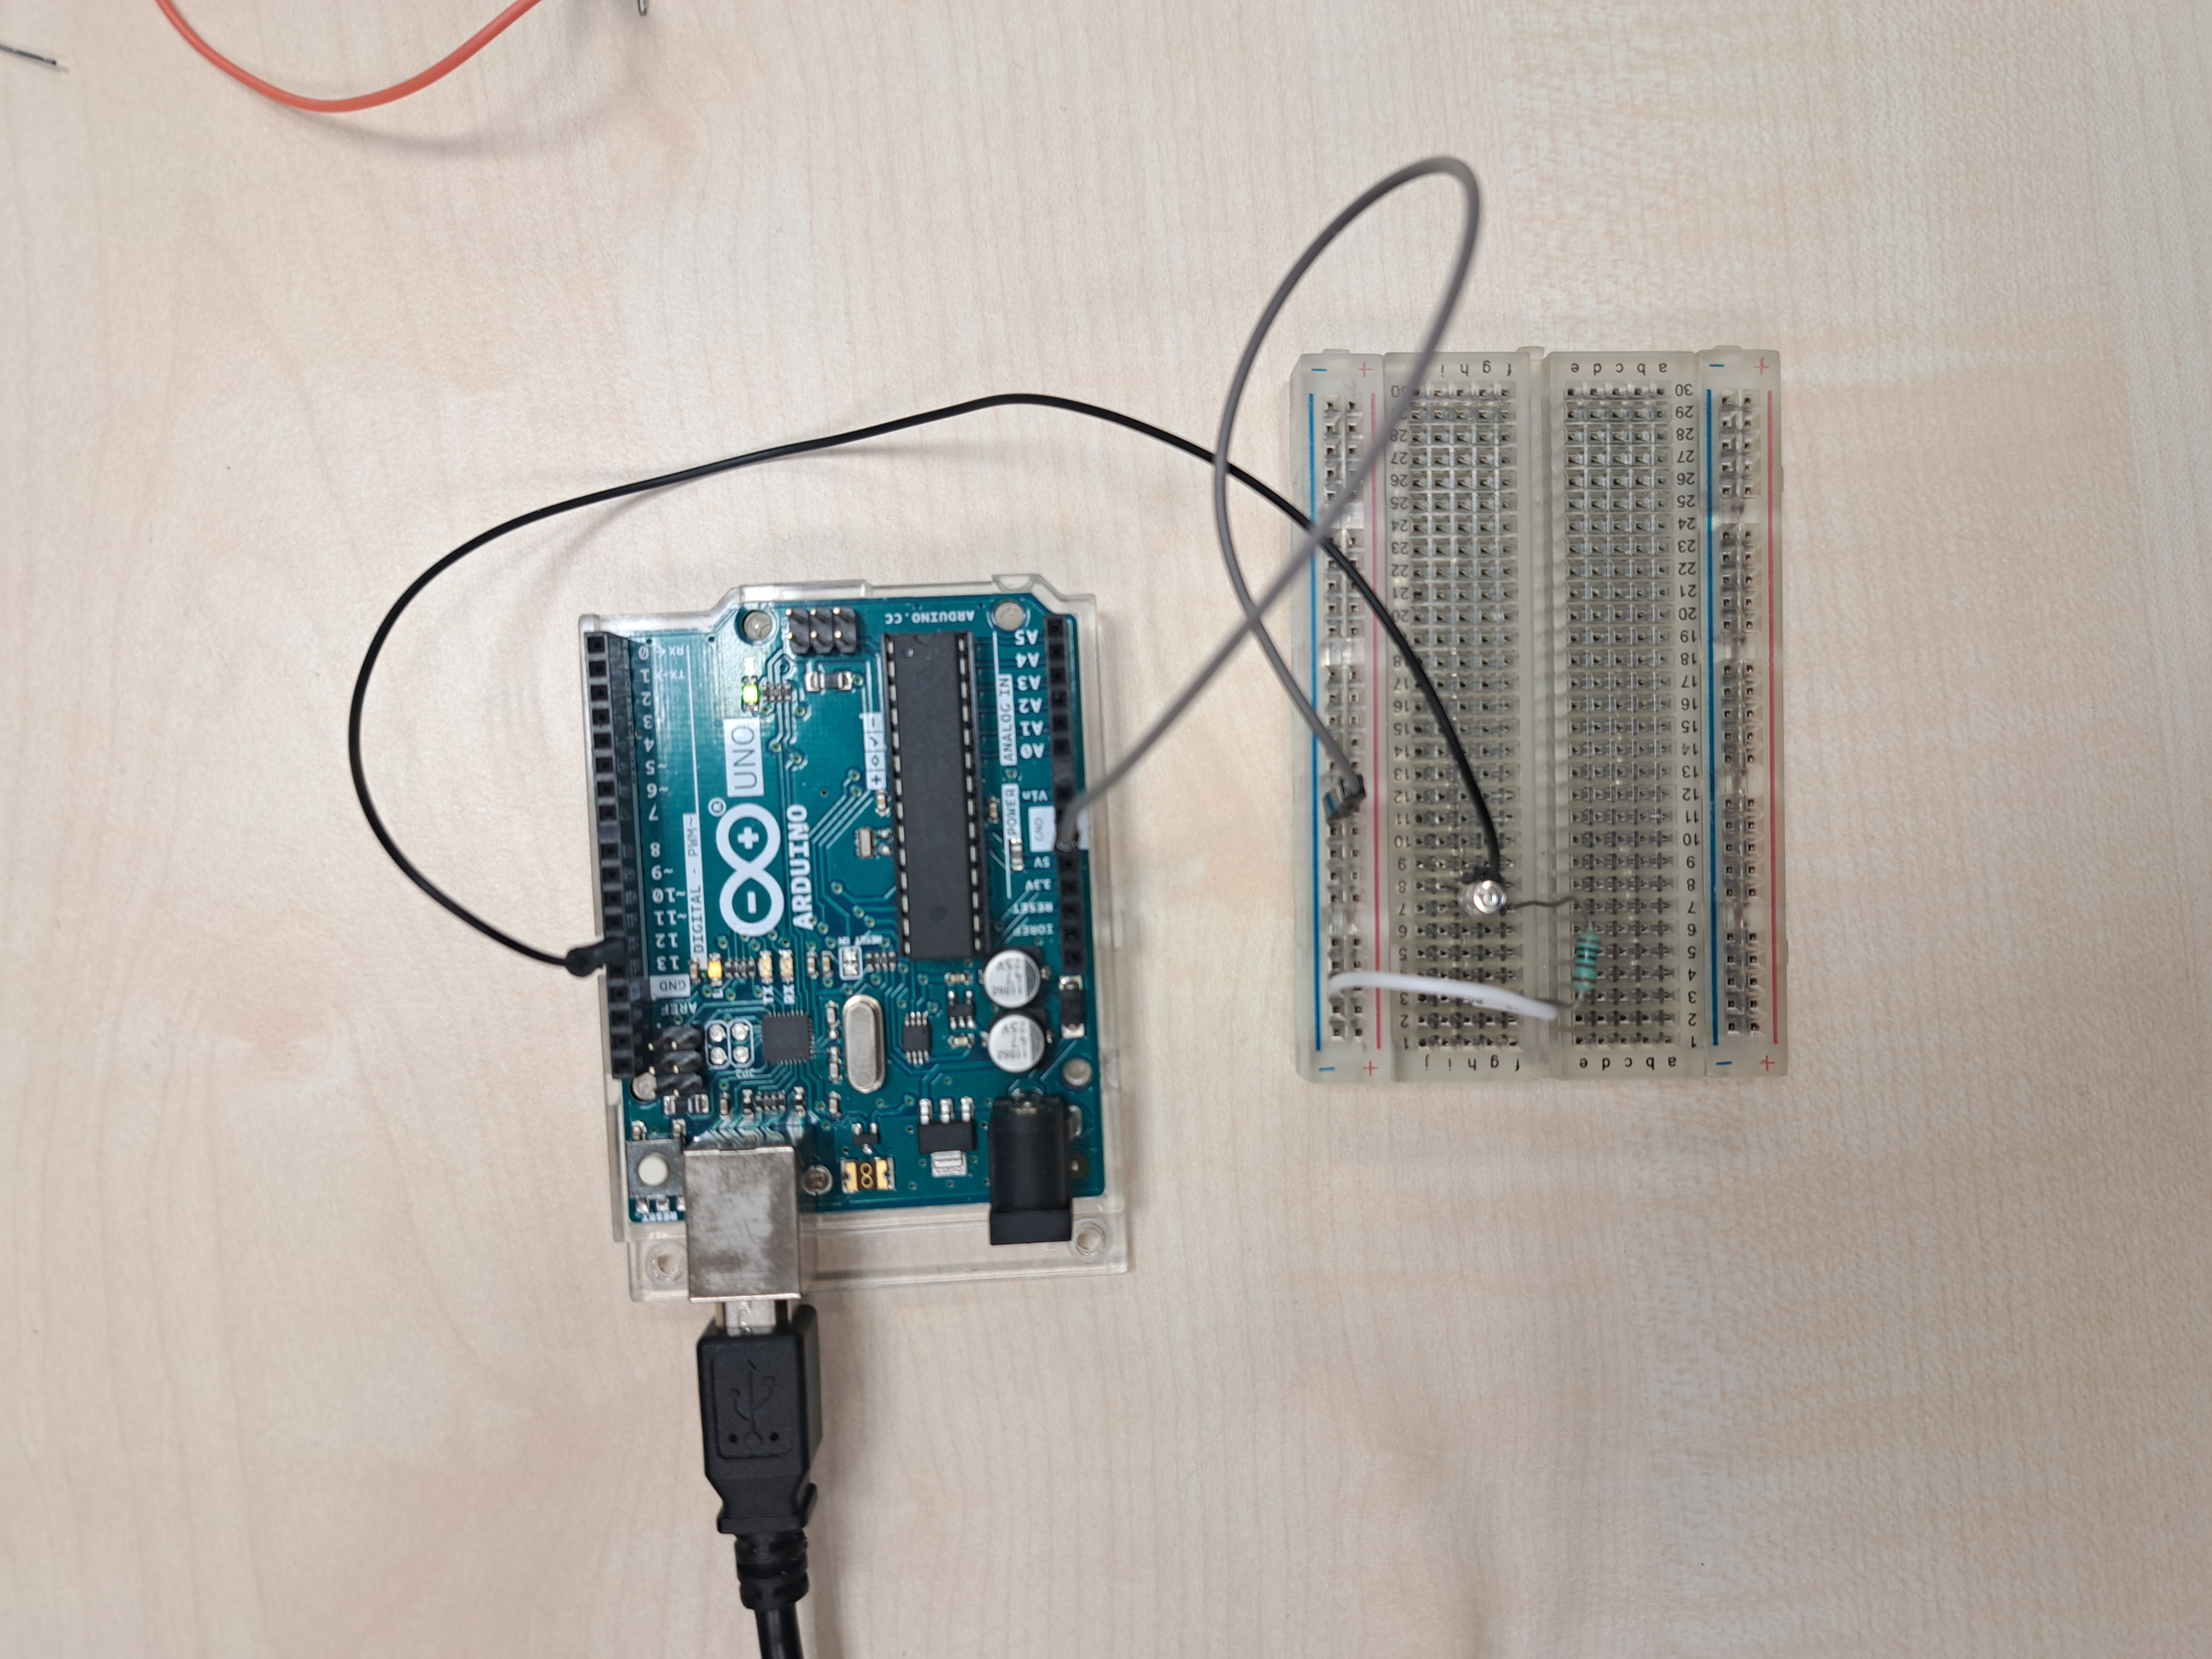
\includegraphics[width=0.5\textwidth]{../temp_figures/exp1/exp1a.jpg}
\end{figure}

\noindent
For this first experiment we set up the \textsf{Arduino Uno} with our Laptop and implemented the following code for the Arduino.

\inputminted[bgcolor=lightgray]{c}{../experiments/exp1a/arduino/1a_sketch.ino}

\noindent
For the Laptop we implemented the following code in Python to read the serial output of the Arduino and save the data.

\inputminted[bgcolor=lightgray]{python}{../experiments/exp1a/python/1a.py}

\subsubsection{Part b}

\begin{figure}[ht]
    \centering
    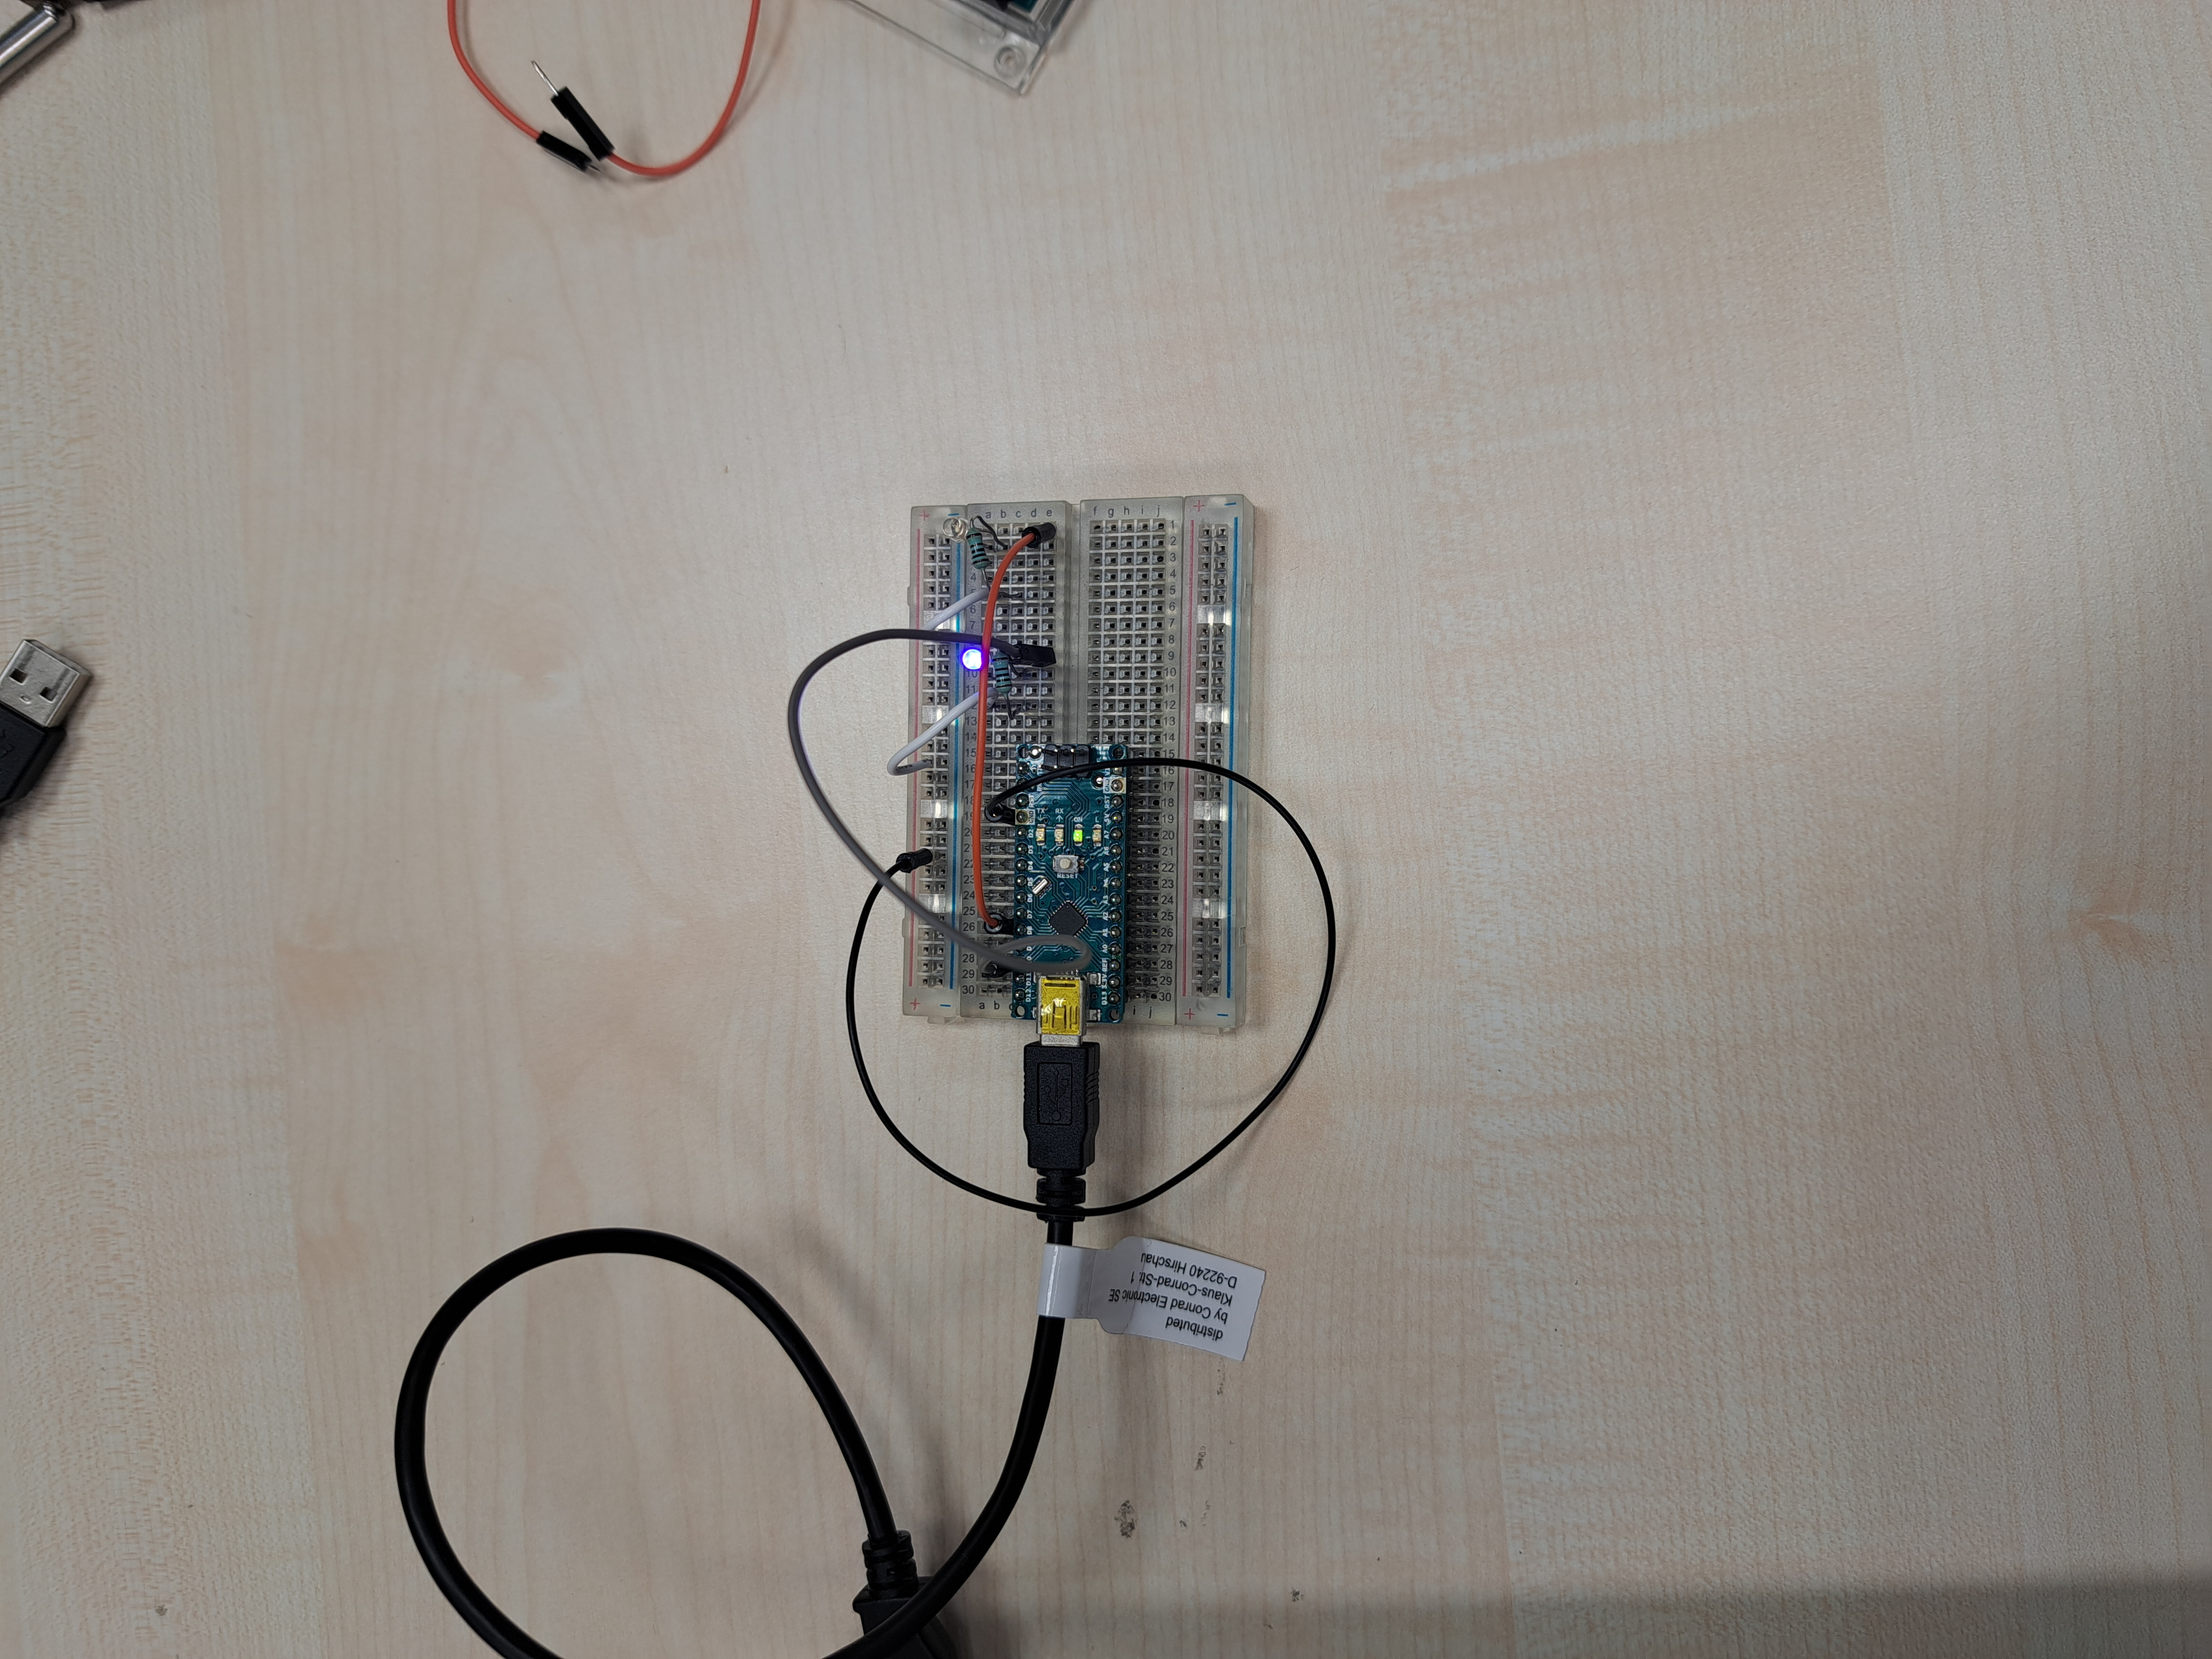
\includegraphics[width=0.5\textwidth]{../temp_figures/exp1/exp1b.jpg}
\end{figure}

\noindent
For the second part of the experiment we set up the \textsf{Arduino Nano} with our Laptop and implemented the following code for the Arduino.

\inputminted[bgcolor=lightgray]{c}{../experiments/exp1b/arduino/1b_sketch.ino}

\noindent
The python code for the Laptop was accordingly adapted to read the serial output of the \textsf{Arduino Nano} and save the data.

\inputminted[bgcolor=lightgray]{python}{../experiments/exp1b/python/1b.py}

\subsubsection{Part c}

For the last part of the experiment we set up the \textsf{Rasperry Pi} to control the LEDs via GPIO Pins.

\inputminted[bgcolor=lightgray]{python}{../experiments/exp1c/python/1c.py}

\subsection{Results}

We managed to adress all the LEDs and save the data. We used this data to plot the State of the LEDs with the time by using \texttt{matplotlib.pyplot.step()}.

\begin{figure}[H]
    \centering
    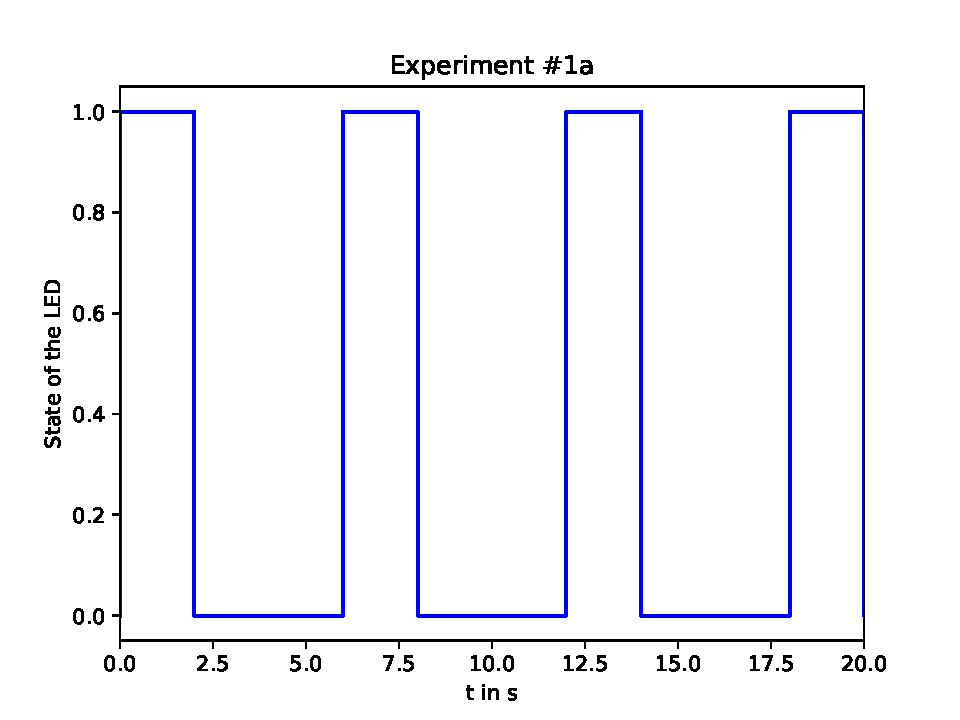
\includegraphics[width=0.7\textwidth]{../temp_figures/exp1/1a.pdf}
    \caption{Plot for 1a}
\end{figure}

\begin{figure}[H]
    \centering
    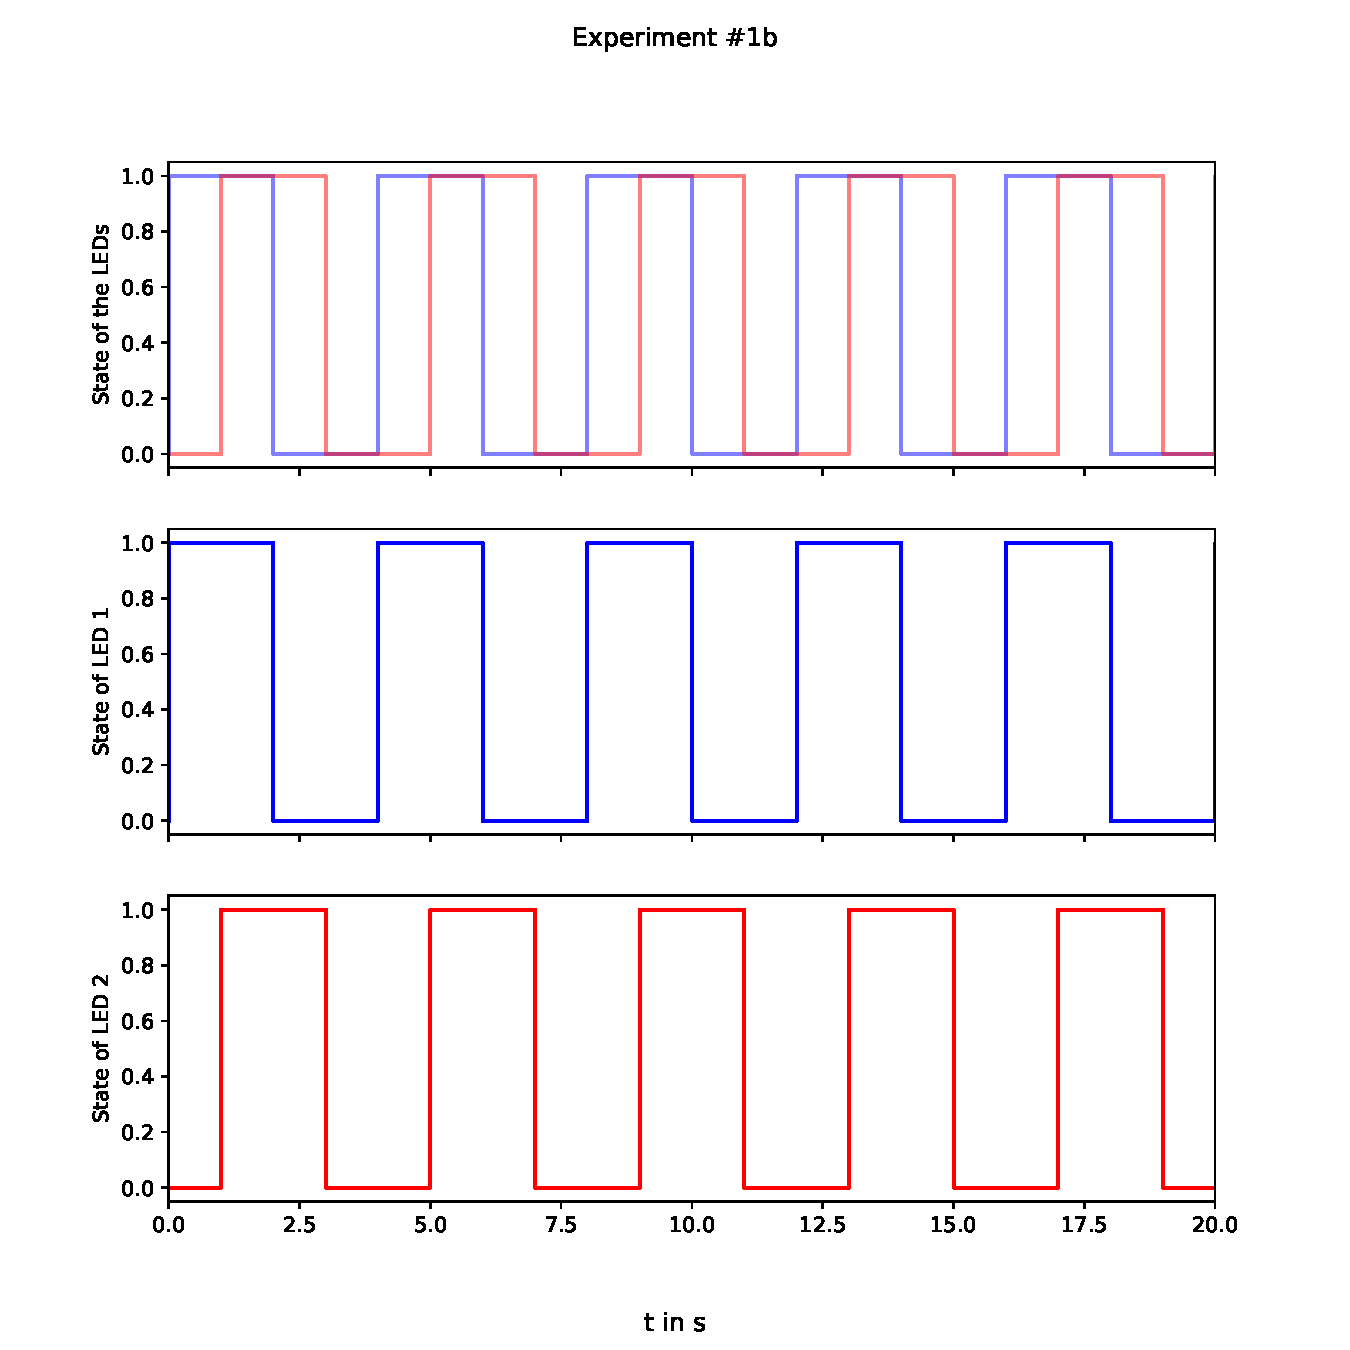
\includegraphics[width=0.7\textwidth]{../temp_figures/exp1/1b.pdf}
    \caption{Plot for 1b}
\end{figure}

\begin{figure}[H]
    \centering
    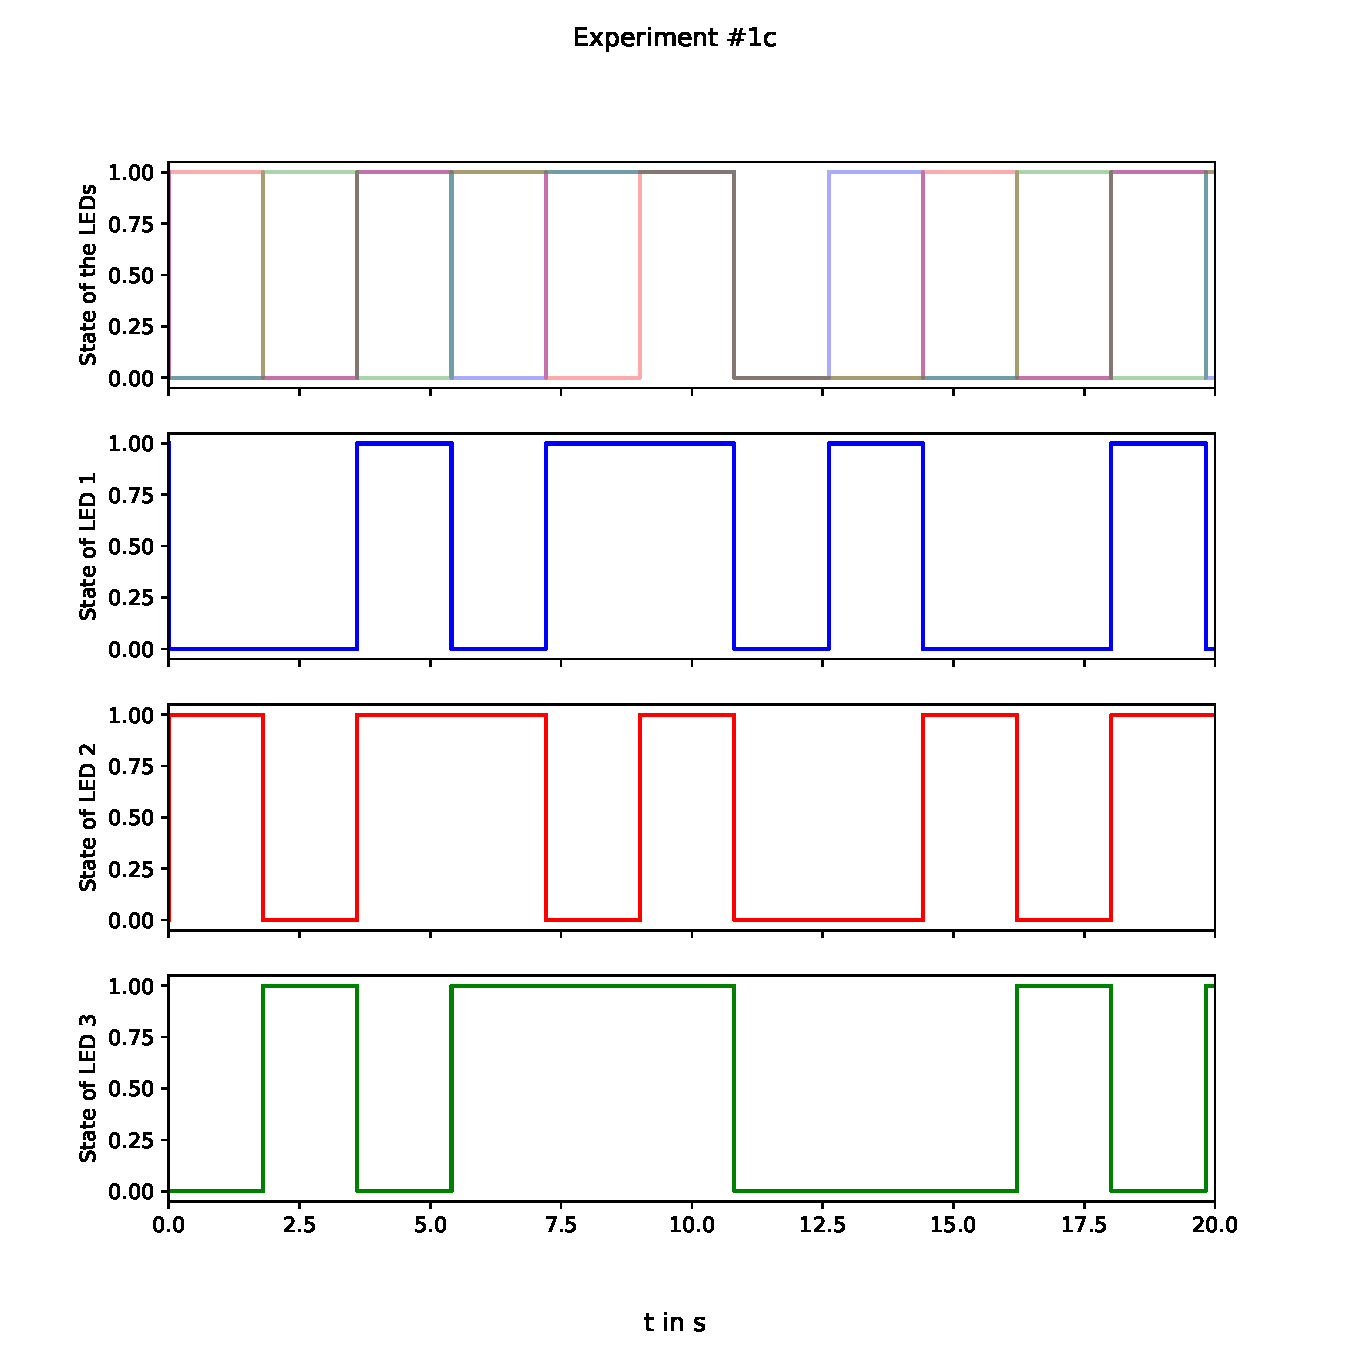
\includegraphics[width=0.7\textwidth]{../temp_figures/exp1/1c.pdf}
    \caption{Plot for 1c}
\end{figure}


\end{document}